\documentclass[1p]{elsarticle_modified}
%\bibliographystyle{elsarticle-num}

%\usepackage[colorlinks]{hyperref}
%\usepackage{abbrmath_seonhwa} %\Abb, \Ascr, \Acal ,\Abf, \Afrak
\usepackage{amsfonts}
\usepackage{amssymb}
\usepackage{amsmath}
\usepackage{amsthm}
\usepackage{scalefnt}
\usepackage{amsbsy}
\usepackage{kotex}
\usepackage{caption}
\usepackage{subfig}
\usepackage{color}
\usepackage{graphicx}
\usepackage{xcolor} %% white, black, red, green, blue, cyan, magenta, yellow
\usepackage{float}
\usepackage{setspace}
\usepackage{hyperref}

\usepackage{tikz}
\usetikzlibrary{arrows}

\usepackage{multirow}
\usepackage{array} % fixed length table
\usepackage{hhline}

%%%%%%%%%%%%%%%%%%%%%
\makeatletter
\renewcommand*\env@matrix[1][\arraystretch]{%
	\edef\arraystretch{#1}%
	\hskip -\arraycolsep
	\let\@ifnextchar\new@ifnextchar
	\array{*\c@MaxMatrixCols c}}
\makeatother %https://tex.stackexchange.com/questions/14071/how-can-i-increase-the-line-spacing-in-a-matrix
%%%%%%%%%%%%%%%

\usepackage[normalem]{ulem}

\newcommand{\msout}[1]{\ifmmode\text{\sout{\ensuremath{#1}}}\else\sout{#1}\fi}
%SOURCE: \msout is \stkout macro in https://tex.stackexchange.com/questions/20609/strikeout-in-math-mode

\newcommand{\cancel}[1]{
	\ifmmode
	{\color{red}\msout{#1}}
	\else
	{\color{red}\sout{#1}}
	\fi
}

\newcommand{\add}[1]{
	{\color{blue}\uwave{#1}}
}

\newcommand{\replace}[2]{
	\ifmmode
	{\color{red}\msout{#1}}{\color{blue}\uwave{#2}}
	\else
	{\color{red}\sout{#1}}{\color{blue}\uwave{#2}}
	\fi
}

\newcommand{\Sol}{\mathcal{S}} %segment
\newcommand{\D}{D} %diagram
\newcommand{\A}{\mathcal{A}} %arc


%%%%%%%%%%%%%%%%%%%%%%%%%%%%%5 test

\def\sl{\operatorname{\textup{SL}}(2,\Cbb)}
\def\psl{\operatorname{\textup{PSL}}(2,\Cbb)}
\def\quan{\mkern 1mu \triangleright \mkern 1mu}

\theoremstyle{definition}
\newtheorem{thm}{Theorem}[section]
\newtheorem{prop}[thm]{Proposition}
\newtheorem{lem}[thm]{Lemma}
\newtheorem{ques}[thm]{Question}
\newtheorem{cor}[thm]{Corollary}
\newtheorem{defn}[thm]{Definition}
\newtheorem{exam}[thm]{Example}
\newtheorem{rmk}[thm]{Remark}
\newtheorem{alg}[thm]{Algorithm}

\newcommand{\I}{\sqrt{-1}}
\begin{document}

%\begin{frontmatter}
%
%\title{Boundary parabolic representations of knots up to 8 crossings}
%
%%% Group authors per affiliation:
%\author{Yunhi Cho} 
%\address{Department of Mathematics, University of Seoul, Seoul, Korea}
%\ead{yhcho@uos.ac.kr}
%
%
%\author{Seonhwa Kim} %\fnref{s_kim}}
%\address{Center for Geometry and Physics, Institute for Basic Science, Pohang, 37673, Korea}
%\ead{ryeona17@ibs.re.kr}
%
%\author{Hyuk Kim}
%\address{Department of Mathematical Sciences, Seoul National University, Seoul 08826, Korea}
%\ead{hyukkim@snu.ac.kr}
%
%\author{Seokbeom Yoon}
%\address{Department of Mathematical Sciences, Seoul National University, Seoul, 08826,  Korea}
%\ead{sbyoon15@snu.ac.kr}
%
%\begin{abstract}
%We find all boundary parabolic representation of knots up to 8 crossings.
%
%\end{abstract}
%\begin{keyword}
%    \MSC[2010] 57M25 
%\end{keyword}
%
%\end{frontmatter}

%\linenumbers
%\tableofcontents
%
\newcommand\colored[1]{\textcolor{white}{\rule[-0.35ex]{0.8em}{1.4ex}}\kern-0.8em\color{red} #1}%
%\newcommand\colored[1]{\textcolor{white}{ #1}\kern-2.17ex	\textcolor{white}{ #1}\kern-1.81ex	\textcolor{white}{ #1}\kern-2.15ex\color{red}#1	}

{\Large $\underline{12n_{0356}~(K12n_{0356})}$}

\setlength{\tabcolsep}{10pt}
\renewcommand{\arraystretch}{1.6}
\vspace{1cm}\begin{tabular}{m{100pt}>{\centering\arraybackslash}m{274pt}}
\multirow{5}{120pt}{
	\centering
	\includegraphics[width=112pt]{../../../GIT/diagram.site/Diagrams/png/2445_12n_0356.png}\\
\ \ \ A knot diagram\footnotemark}&
\allowdisplaybreaks
\textbf{Linearized knot diagam} \\
\cline{2-2}
 &
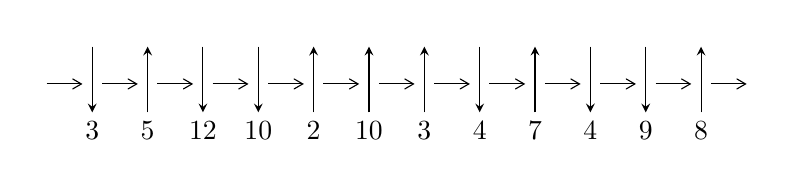
\begin{tikzpicture}[x=20pt, y=17pt]
	% nodes
	\node (C0) at (0, 0) {};
	\node (C1) at (1, 0) {};
	\node (C1U) at (1, +1) {};
	\node (C1D) at (1, -1) {3};

	\node (C2) at (2, 0) {};
	\node (C2U) at (2, +1) {};
	\node (C2D) at (2, -1) {5};

	\node (C3) at (3, 0) {};
	\node (C3U) at (3, +1) {};
	\node (C3D) at (3, -1) {12};

	\node (C4) at (4, 0) {};
	\node (C4U) at (4, +1) {};
	\node (C4D) at (4, -1) {10};

	\node (C5) at (5, 0) {};
	\node (C5U) at (5, +1) {};
	\node (C5D) at (5, -1) {2};

	\node (C6) at (6, 0) {};
	\node (C6U) at (6, +1) {};
	\node (C6D) at (6, -1) {10};

	\node (C7) at (7, 0) {};
	\node (C7U) at (7, +1) {};
	\node (C7D) at (7, -1) {3};

	\node (C8) at (8, 0) {};
	\node (C8U) at (8, +1) {};
	\node (C8D) at (8, -1) {4};

	\node (C9) at (9, 0) {};
	\node (C9U) at (9, +1) {};
	\node (C9D) at (9, -1) {7};

	\node (C10) at (10, 0) {};
	\node (C10U) at (10, +1) {};
	\node (C10D) at (10, -1) {4};

	\node (C11) at (11, 0) {};
	\node (C11U) at (11, +1) {};
	\node (C11D) at (11, -1) {9};

	\node (C12) at (12, 0) {};
	\node (C12U) at (12, +1) {};
	\node (C12D) at (12, -1) {8};
	\node (C13) at (13, 0) {};

	% arrows
	\draw[->,>={angle 60}]
	(C0) edge (C1) (C1) edge (C2) (C2) edge (C3) (C3) edge (C4) (C4) edge (C5) (C5) edge (C6) (C6) edge (C7) (C7) edge (C8) (C8) edge (C9) (C9) edge (C10) (C10) edge (C11) (C11) edge (C12) (C12) edge (C13) ;	\draw[->,>=stealth]
	(C1U) edge (C1D) (C2D) edge (C2U) (C3U) edge (C3D) (C4U) edge (C4D) (C5D) edge (C5U) (C6D) edge (C6U) (C7D) edge (C7U) (C8U) edge (C8D) (C9D) edge (C9U) (C10U) edge (C10D) (C11U) edge (C11D) (C12D) edge (C12U) ;
	\end{tikzpicture} \\
\hhline{~~} \\& 
\textbf{Solving Sequence} \\ \cline{2-2} 
 &
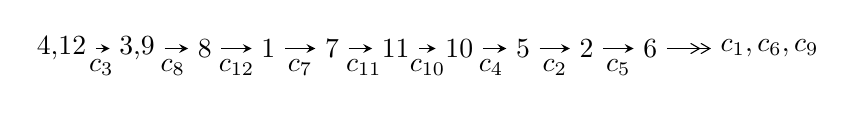
\begin{tikzpicture}[x=23pt, y=7pt]
	% node
	\node (A0) at (-1/8, 0) {4,12};
	\node (A1) at (17/16, 0) {3,9};
	\node (A2) at (17/8, 0) {8};
	\node (A3) at (25/8, 0) {1};
	\node (A4) at (33/8, 0) {7};
	\node (A5) at (41/8, 0) {11};
	\node (A6) at (49/8, 0) {10};
	\node (A7) at (57/8, 0) {5};
	\node (A8) at (65/8, 0) {2};
	\node (A9) at (73/8, 0) {6};
	\node (C1) at (1/2, -1) {$c_{3}$};
	\node (C2) at (13/8, -1) {$c_{8}$};
	\node (C3) at (21/8, -1) {$c_{12}$};
	\node (C4) at (29/8, -1) {$c_{7}$};
	\node (C5) at (37/8, -1) {$c_{11}$};
	\node (C6) at (45/8, -1) {$c_{10}$};
	\node (C7) at (53/8, -1) {$c_{4}$};
	\node (C8) at (61/8, -1) {$c_{2}$};
	\node (C9) at (69/8, -1) {$c_{5}$};
	\node (A10) at (11, 0) {$c_{1},c_{6},c_{9}$};

	% edge
	\draw[->,>=stealth]	
	(A0) edge (A1) (A1) edge (A2) (A2) edge (A3) (A3) edge (A4) (A4) edge (A5) (A5) edge (A6) (A6) edge (A7) (A7) edge (A8) (A8) edge (A9) ;
	\draw[->>,>={angle 60}]	
	(A9) edge (A10);
\end{tikzpicture} \\ 

\end{tabular} \\

\footnotetext{
The image of knot diagram is generated by the software ``\textbf{Draw programme}" developed by Andrew Bartholomew(\url{http://www.layer8.co.uk/maths/draw/index.htm\#Running-draw}), where we modified some parts for our purpose(\url{https://github.com/CATsTAILs/LinksPainter}).
}\phantom \\ \newline 
\centering \textbf{Ideals for irreducible components\footnotemark of $X_{\text{par}}$} 
 
\begin{align*}
I^u_{1}&=\langle 
7.95983\times10^{44} u^{41}-1.50155\times10^{45} u^{40}+\cdots+1.14909\times10^{45} b-1.16386\times10^{46},\\
\phantom{I^u_{1}}&\phantom{= \langle  }6.40800\times10^{45} u^{41}-3.37761\times10^{44} u^{40}+\cdots+3.44727\times10^{45} a-2.38350\times10^{46},\;u^{42}+6 u^{40}+\cdots-4 u+3\rangle \\
I^u_{2}&=\langle 
b-1,\;a+1,\;u^2+u+1\rangle \\
I^u_{3}&=\langle 
- u^9-3 u^7-5 u^5- u^4-10 u^3- u^2+b-6 u,\\
\phantom{I^u_{3}}&\phantom{= \langle  }-126 u^9-4 u^8-339 u^7-31 u^6-519 u^5-187 u^4-1073 u^3-183 u^2+85 a-564 u-111,\\
\phantom{I^u_{3}}&\phantom{= \langle  }u^{10}+3 u^8+5 u^6+u^5+10 u^4+u^3+7 u^2+1\rangle \\
\\
\end{align*}
\raggedright * 3 irreducible components of $\dim_{\mathbb{C}}=0$, with total 54 representations.\\
\footnotetext{All coefficients of polynomials are rational numbers. But the coefficients are sometimes approximated in decimal forms when there is not enough margin.}
\newpage
\renewcommand{\arraystretch}{1}
\centering \section*{I. $I^u_{1}= \langle 7.96\times10^{44} u^{41}-1.50\times10^{45} u^{40}+\cdots+1.15\times10^{45} b-1.16\times10^{46},\;6.41\times10^{45} u^{41}-3.38\times10^{44} u^{40}+\cdots+3.45\times10^{45} a-2.38\times10^{46},\;u^{42}+6 u^{40}+\cdots-4 u+3 \rangle$}
\flushleft \textbf{(i) Arc colorings}\\
\begin{tabular}{m{7pt} m{180pt} m{7pt} m{180pt} }
\flushright $a_{4}=$&$\begin{pmatrix}1\\0\end{pmatrix}$ \\
\flushright $a_{12}=$&$\begin{pmatrix}0\\u\end{pmatrix}$ \\
\flushright $a_{3}=$&$\begin{pmatrix}1\\- u^2\end{pmatrix}$ \\
\flushright $a_{9}=$&$\begin{pmatrix}-1.85886 u^{41}+0.0979791 u^{40}+\cdots-27.6246 u+6.91416\\-0.692707 u^{41}+1.30673 u^{40}+\cdots-11.4825 u+10.1285\end{pmatrix}$ \\
\flushright $a_{8}=$&$\begin{pmatrix}-2.55157 u^{41}+1.40471 u^{40}+\cdots-39.1071 u+17.0427\\-0.692707 u^{41}+1.30673 u^{40}+\cdots-11.4825 u+10.1285\end{pmatrix}$ \\
\flushright $a_{1}=$&$\begin{pmatrix}0.832926 u^{41}-0.346814 u^{40}+\cdots+10.5076 u+6.09743\\-0.155548 u^{41}+0.571430 u^{40}+\cdots-4.77363 u+6.26450\end{pmatrix}$ \\
\flushright $a_{7}=$&$\begin{pmatrix}-2.86555 u^{41}+0.463510 u^{40}+\cdots-40.8981 u+11.1283\\-0.435280 u^{41}+1.07479 u^{40}+\cdots-8.65966 u+7.30494\end{pmatrix}$ \\
\flushright $a_{11}=$&$\begin{pmatrix}0.0541962 u^{41}-0.173110 u^{40}+\cdots+5.05694 u+7.82335\\0.934277 u^{41}-0.745135 u^{40}+\cdots+12.2243 u-7.99042\end{pmatrix}$ \\
\flushright $a_{10}=$&$\begin{pmatrix}0.988473 u^{41}-0.918245 u^{40}+\cdots+17.2813 u-0.167070\\0.934277 u^{41}-0.745135 u^{40}+\cdots+12.2243 u-7.99042\end{pmatrix}$ \\
\flushright $a_{5}=$&$\begin{pmatrix}2.78167 u^{41}-0.519929 u^{40}+\cdots+10.7131 u-6.92196\\0.763818 u^{41}-0.555089 u^{40}+\cdots+9.41655 u-4.17445\end{pmatrix}$ \\
\flushright $a_{2}=$&$\begin{pmatrix}1.26821 u^{41}-1.42161 u^{40}+\cdots+19.1673 u-1.20751\\0.308673 u^{41}+0.214746 u^{40}+\cdots+0.831385 u+3.04011\end{pmatrix}$ \\
\flushright $a_{6}=$&$\begin{pmatrix}4.26347 u^{41}-3.57388 u^{40}+\cdots+63.8196 u-31.1222\\2.53749 u^{41}-2.17142 u^{40}+\cdots+37.6429 u-19.2215\end{pmatrix}$\\&\end{tabular}
\flushleft \textbf{(ii) Obstruction class $= -1$}\\~\\
\flushleft \textbf{(iii) Cusp Shapes $= 11.6391 u^{41}-2.74474 u^{40}+\cdots+169.526 u-46.9504$}\\~\\
\newpage\renewcommand{\arraystretch}{1}
\flushleft \textbf{(iv) u-Polynomials at the component}\newline \\
\begin{tabular}{m{50pt}|m{274pt}}
Crossings & \hspace{64pt}u-Polynomials at each crossing \\
\hline $$\begin{aligned}c_{1}\end{aligned}$$&$\begin{aligned}
&u^{42}+12 u^{41}+\cdots+230 u+9
\end{aligned}$\\
\hline $$\begin{aligned}c_{2},c_{5}\end{aligned}$$&$\begin{aligned}
&u^{42}+6 u^{40}+\cdots+4 u+3
\end{aligned}$\\
\hline $$\begin{aligned}c_{3}\end{aligned}$$&$\begin{aligned}
&u^{42}+6 u^{40}+\cdots-4 u+3
\end{aligned}$\\
\hline $$\begin{aligned}c_{4},c_{10}\end{aligned}$$&$\begin{aligned}
&u^{42}+14 u^{40}+\cdots-792 u+172
\end{aligned}$\\
\hline $$\begin{aligned}c_{6},c_{9}\end{aligned}$$&$\begin{aligned}
&u^{42}+3 u^{41}+\cdots+1471 u+111
\end{aligned}$\\
\hline $$\begin{aligned}c_{7}\end{aligned}$$&$\begin{aligned}
&u^{42}+u^{41}+\cdots+47 u+99
\end{aligned}$\\
\hline $$\begin{aligned}c_{8}\end{aligned}$$&$\begin{aligned}
&u^{42}+u^{41}+\cdots-131 u+111
\end{aligned}$\\
\hline $$\begin{aligned}c_{11}\end{aligned}$$&$\begin{aligned}
&u^{42}-3 u^{41}+\cdots-1471 u+111
\end{aligned}$\\
\hline $$\begin{aligned}c_{12}\end{aligned}$$&$\begin{aligned}
&u^{42}+14 u^{40}+\cdots+792 u+172
\end{aligned}$\\
\hline
\end{tabular}\\~\\
\newpage\renewcommand{\arraystretch}{1}
\flushleft \textbf{(v) Riley Polynomials at the component}\newline \\
\begin{tabular}{m{50pt}|m{274pt}}
Crossings & \hspace{64pt}Riley Polynomials at each crossing \\
\hline $$\begin{aligned}c_{1}\end{aligned}$$&$\begin{aligned}
&y^{42}+44 y^{41}+\cdots+254 y+81
\end{aligned}$\\
\hline $$\begin{aligned}c_{2},c_{3},c_{5}\end{aligned}$$&$\begin{aligned}
&y^{42}+12 y^{41}+\cdots+230 y+9
\end{aligned}$\\
\hline $$\begin{aligned}c_{4},c_{10},c_{12}\end{aligned}$$&$\begin{aligned}
&y^{42}+28 y^{41}+\cdots+8448 y+29584
\end{aligned}$\\
\hline $$\begin{aligned}c_{6},c_{9},c_{11}\end{aligned}$$&$\begin{aligned}
&y^{42}-27 y^{41}+\cdots+55937 y+12321
\end{aligned}$\\
\hline $$\begin{aligned}c_{7}\end{aligned}$$&$\begin{aligned}
&y^{42}+21 y^{41}+\cdots+383891 y+9801
\end{aligned}$\\
\hline $$\begin{aligned}c_{8}\end{aligned}$$&$\begin{aligned}
&y^{42}-29 y^{41}+\cdots+95171 y+12321
\end{aligned}$\\
\hline
\end{tabular}\\~\\
\newpage\flushleft \textbf{(vi) Complex Volumes and Cusp Shapes}
$$\begin{array}{c|c|c}  
\text{Solutions to }I^u_{1}& \I (\text{vol} + \sqrt{-1}CS) & \text{Cusp shape}\\
 \hline 
\begin{aligned}
u &= -0.544383 + 0.863324 I \\
a &= -0.51188 + 1.32823 I \\
b &= -0.497540 + 0.008587 I\end{aligned}
 & \phantom{-}2.42641 - 0.18863 I & \phantom{-}3.24251 - 0.93757 I \\ \hline\begin{aligned}
u &= -0.544383 - 0.863324 I \\
a &= -0.51188 - 1.32823 I \\
b &= -0.497540 - 0.008587 I\end{aligned}
 & \phantom{-}2.42641 + 0.18863 I & \phantom{-}3.24251 + 0.93757 I \\ \hline\begin{aligned}
u &= -0.687915 + 0.682286 I \\
a &= \phantom{-}1.102770 - 0.213792 I \\
b &= -1.75734 + 0.28348 I\end{aligned}
 & \phantom{-}1.70620 + 4.86322 I & \phantom{-}2.22045 - 7.40969 I \\ \hline\begin{aligned}
u &= -0.687915 - 0.682286 I \\
a &= \phantom{-}1.102770 + 0.213792 I \\
b &= -1.75734 - 0.28348 I\end{aligned}
 & \phantom{-}1.70620 - 4.86322 I & \phantom{-}2.22045 + 7.40969 I \\ \hline\begin{aligned}
u &= \phantom{-}0.750317 + 0.769897 I \\
a &= \phantom{-}1.340840 - 0.353204 I \\
b &= -1.37469 - 1.08554 I\end{aligned}
 & -3.29363 - 5.13657 I & -2.33265 + 8.72582 I \\ \hline\begin{aligned}
u &= \phantom{-}0.750317 - 0.769897 I \\
a &= \phantom{-}1.340840 + 0.353204 I \\
b &= -1.37469 + 1.08554 I\end{aligned}
 & -3.29363 + 5.13657 I & -2.33265 - 8.72582 I \\ \hline\begin{aligned}
u &= -0.932214 + 0.569996 I \\
a &= -1.037210 - 0.591475 I \\
b &= \phantom{-}0.860453 - 0.527673 I\end{aligned}
 & -3.75518 + 1.50447 I & -4.91299 + 0.56780 I \\ \hline\begin{aligned}
u &= -0.932214 - 0.569996 I \\
a &= -1.037210 + 0.591475 I \\
b &= \phantom{-}0.860453 + 0.527673 I\end{aligned}
 & -3.75518 - 1.50447 I & -4.91299 - 0.56780 I \\ \hline\begin{aligned}
u &= -0.144161 + 0.853584 I \\
a &= -1.010980 - 0.281506 I \\
b &= \phantom{-}0.414095 + 0.757109 I\end{aligned}
 & \phantom{-}0.95566 + 2.59332 I & \phantom{-}5.16066 - 5.00921 I \\ \hline\begin{aligned}
u &= -0.144161 - 0.853584 I \\
a &= -1.010980 + 0.281506 I \\
b &= \phantom{-}0.414095 - 0.757109 I\end{aligned}
 & \phantom{-}0.95566 - 2.59332 I & \phantom{-}5.16066 + 5.00921 I\\
 \hline 
 \end{array}$$\newpage$$\begin{array}{c|c|c}  
\text{Solutions to }I^u_{1}& \I (\text{vol} + \sqrt{-1}CS) & \text{Cusp shape}\\
 \hline 
\begin{aligned}
u &= \phantom{-}0.547178 + 0.657889 I \\
a &= \phantom{-}1.21496 + 1.75367 I \\
b &= \phantom{-}0.157769 - 0.348092 I\end{aligned}
 & \phantom{-}3.29363 - 5.13657 I & \phantom{-}2.33265 + 8.72582 I \\ \hline\begin{aligned}
u &= \phantom{-}0.547178 - 0.657889 I \\
a &= \phantom{-}1.21496 - 1.75367 I \\
b &= \phantom{-}0.157769 + 0.348092 I\end{aligned}
 & \phantom{-}3.29363 + 5.13657 I & \phantom{-}2.33265 - 8.72582 I \\ \hline\begin{aligned}
u &= \phantom{-}0.402523 + 0.735634 I \\
a &= -1.213870 - 0.554358 I \\
b &= \phantom{-}1.46993 + 0.46496 I\end{aligned}
 & \phantom{-}3.75518 + 1.50447 I & \phantom{-}4.91299 + 0.56780 I \\ \hline\begin{aligned}
u &= \phantom{-}0.402523 - 0.735634 I \\
a &= -1.213870 + 0.554358 I \\
b &= \phantom{-}1.46993 - 0.46496 I\end{aligned}
 & \phantom{-}3.75518 - 1.50447 I & \phantom{-}4.91299 - 0.56780 I \\ \hline\begin{aligned}
u &= \phantom{-}0.618713 + 1.043480 I \\
a &= \phantom{-}0.248973 - 0.791074 I \\
b &= -1.309910 + 0.260236 I\end{aligned}
 & -2.42641 - 0.18863 I & -3.24251 - 0.93757 I \\ \hline\begin{aligned}
u &= \phantom{-}0.618713 - 1.043480 I \\
a &= \phantom{-}0.248973 + 0.791074 I \\
b &= -1.309910 - 0.260236 I\end{aligned}
 & -2.42641 + 0.18863 I & -3.24251 + 0.93757 I \\ \hline\begin{aligned}
u &= \phantom{-}0.831964 + 0.909186 I \\
a &= \phantom{-}1.28883 - 0.94404 I \\
b &= -1.80526 - 0.30079 I\end{aligned}
 & -5.39497 - 3.10535 I & -10.05216 + 0. I\phantom{ +0.000000I} \\ \hline\begin{aligned}
u &= \phantom{-}0.831964 - 0.909186 I \\
a &= \phantom{-}1.28883 + 0.94404 I \\
b &= -1.80526 + 0.30079 I\end{aligned}
 & -5.39497 + 3.10535 I & -10.05216 + 0. I\phantom{ +0.000000I} \\ \hline\begin{aligned}
u &= -1.042840 + 0.697476 I \\
a &= \phantom{-}0.494099 + 0.769179 I \\
b &= -1.144430 - 0.016547 I\end{aligned}
 & \phantom{-0.000000 } -0.206317 I & \phantom{-0.000000 } 0 \\ \hline\begin{aligned}
u &= -1.042840 - 0.697476 I \\
a &= \phantom{-}0.494099 - 0.769179 I \\
b &= -1.144430 + 0.016547 I\end{aligned}
 & \phantom{-0.000000 -}0.206317 I & \phantom{-0.000000 } 0\\
 \hline 
 \end{array}$$\newpage$$\begin{array}{c|c|c}  
\text{Solutions to }I^u_{1}& \I (\text{vol} + \sqrt{-1}CS) & \text{Cusp shape}\\
 \hline 
\begin{aligned}
u &= \phantom{-}0.033933 + 0.665190 I \\
a &= -0.60540 + 2.41235 I \\
b &= -0.141969 + 1.363470 I\end{aligned}
 & \phantom{-}5.39497 + 3.10535 I & \phantom{-}10.05216 - 0.84923 I \\ \hline\begin{aligned}
u &= \phantom{-}0.033933 - 0.665190 I \\
a &= -0.60540 - 2.41235 I \\
b &= -0.141969 - 1.363470 I\end{aligned}
 & \phantom{-}5.39497 - 3.10535 I & \phantom{-}10.05216 + 0.84923 I \\ \hline\begin{aligned}
u &= \phantom{-}1.122240 + 0.748923 I \\
a &= -0.720260 + 0.883365 I \\
b &= \phantom{-}1.377720 - 0.195992 I\end{aligned}
 & -1.23530 + 7.11550 I & \phantom{-0.000000 } 0 \\ \hline\begin{aligned}
u &= \phantom{-}1.122240 - 0.748923 I \\
a &= -0.720260 - 0.883365 I \\
b &= \phantom{-}1.377720 + 0.195992 I\end{aligned}
 & -1.23530 - 7.11550 I & \phantom{-0.000000 } 0 \\ \hline\begin{aligned}
u &= \phantom{-}0.984944 + 0.968446 I \\
a &= -0.621355 + 0.424387 I \\
b &= \phantom{-}1.41482 + 0.57562 I\end{aligned}
 & -8.49949 - 3.58541 I & \phantom{-0.000000 } 0 \\ \hline\begin{aligned}
u &= \phantom{-}0.984944 - 0.968446 I \\
a &= -0.621355 - 0.424387 I \\
b &= \phantom{-}1.41482 - 0.57562 I\end{aligned}
 & -8.49949 + 3.58541 I & \phantom{-0.000000 } 0 \\ \hline\begin{aligned}
u &= -0.360297 + 0.499277 I \\
a &= -0.145220 + 0.355309 I \\
b &= -0.293588 + 0.434809 I\end{aligned}
 & \phantom{-0.000000 -}1.15367 I & \phantom{-0.000000 } 0. - 5.79196 I \\ \hline\begin{aligned}
u &= -0.360297 - 0.499277 I \\
a &= -0.145220 - 0.355309 I \\
b &= -0.293588 - 0.434809 I\end{aligned}
 & \phantom{-0.000000 } -1.15367 I & \phantom{-0.000000 -}0. + 5.79196 I \\ \hline\begin{aligned}
u &= \phantom{-}0.129278 + 0.581586 I \\
a &= \phantom{-}0.221386 + 0.378940 I \\
b &= \phantom{-}0.01026 - 2.64515 I\end{aligned}
 & \phantom{-}5.05194 - 3.77462 I & \phantom{-}11.6382 + 10.3724 I \\ \hline\begin{aligned}
u &= \phantom{-}0.129278 - 0.581586 I \\
a &= \phantom{-}0.221386 - 0.378940 I \\
b &= \phantom{-}0.01026 + 2.64515 I\end{aligned}
 & \phantom{-}5.05194 + 3.77462 I & \phantom{-}11.6382 - 10.3724 I\\
 \hline 
 \end{array}$$\newpage$$\begin{array}{c|c|c}  
\text{Solutions to }I^u_{1}& \I (\text{vol} + \sqrt{-1}CS) & \text{Cusp shape}\\
 \hline 
\begin{aligned}
u &= -0.865461 + 1.109310 I \\
a &= \phantom{-}0.989347 + 0.290574 I \\
b &= -1.56337 + 0.89130 I\end{aligned}
 & \phantom{-}1.23530 + 7.11550 I & \phantom{-0.000000 } 0 \\ \hline\begin{aligned}
u &= -0.865461 - 1.109310 I \\
a &= \phantom{-}0.989347 - 0.290574 I \\
b &= -1.56337 - 0.89130 I\end{aligned}
 & \phantom{-}1.23530 - 7.11550 I & \phantom{-0.000000 } 0 \\ \hline\begin{aligned}
u &= -1.05197 + 0.94991 I \\
a &= -1.180020 - 0.609379 I \\
b &= \phantom{-}1.382870 - 0.244233 I\end{aligned}
 & -5.05194 + 3.77462 I & \phantom{-0.000000 } 0 \\ \hline\begin{aligned}
u &= -1.05197 - 0.94991 I \\
a &= -1.180020 + 0.609379 I \\
b &= \phantom{-}1.382870 + 0.244233 I\end{aligned}
 & -5.05194 - 3.77462 I & \phantom{-0.000000 } 0 \\ \hline\begin{aligned}
u &= \phantom{-}0.89172 + 1.13300 I \\
a &= -1.161700 + 0.418276 I \\
b &= \phantom{-}1.72271 + 0.83595 I\end{aligned}
 & \phantom{-0.000000 } -14.3453 I & \phantom{-0.000000 } 0 \\ \hline\begin{aligned}
u &= \phantom{-}0.89172 - 1.13300 I \\
a &= -1.161700 - 0.418276 I \\
b &= \phantom{-}1.72271 - 0.83595 I\end{aligned}
 & \phantom{-0.000000 -}14.3453 I & \phantom{-0.000000 } 0 \\ \hline\begin{aligned}
u &= -0.76555 + 1.23008 I \\
a &= -0.662962 - 0.381871 I \\
b &= \phantom{-}1.242360 - 0.087577 I\end{aligned}
 & -1.70620 + 4.86322 I & \phantom{-0.000000 } 0 \\ \hline\begin{aligned}
u &= -0.76555 - 1.23008 I \\
a &= -0.662962 + 0.381871 I \\
b &= \phantom{-}1.242360 + 0.087577 I\end{aligned}
 & -1.70620 - 4.86322 I & \phantom{-0.000000 } 0 \\ \hline\begin{aligned}
u &= \phantom{-}0.157972 + 0.382405 I \\
a &= \phantom{-}3.18352 - 0.59179 I \\
b &= -0.795555 - 0.090965 I\end{aligned}
 & -0.95566 - 2.59332 I & -5.16066 + 5.00921 I \\ \hline\begin{aligned}
u &= \phantom{-}0.157972 - 0.382405 I \\
a &= \phantom{-}3.18352 + 0.59179 I \\
b &= -0.795555 + 0.090965 I\end{aligned}
 & -0.95566 + 2.59332 I & -5.16066 - 5.00921 I\\
 \hline 
 \end{array}$$\newpage$$\begin{array}{c|c|c}  
\text{Solutions to }I^u_{1}& \I (\text{vol} + \sqrt{-1}CS) & \text{Cusp shape}\\
 \hline 
\begin{aligned}
u &= -0.07599 + 1.62893 I \\
a &= -0.047185 + 0.419190 I \\
b &= \phantom{-}0.130648 - 0.204139 I\end{aligned}
 & \phantom{-}8.49949 + 3.58541 I & \phantom{-0.000000 } 0 \\ \hline\begin{aligned}
u &= -0.07599 - 1.62893 I \\
a &= -0.047185 - 0.419190 I \\
b &= \phantom{-}0.130648 + 0.204139 I\end{aligned}
 & \phantom{-}8.49949 - 3.58541 I & \phantom{-0.000000 } 0\\
 \hline 
 \end{array}$$\newpage\newpage\renewcommand{\arraystretch}{1}
\centering \section*{II. $I^u_{2}= \langle b-1,\;a+1,\;u^2+u+1 \rangle$}
\flushleft \textbf{(i) Arc colorings}\\
\begin{tabular}{m{7pt} m{180pt} m{7pt} m{180pt} }
\flushright $a_{4}=$&$\begin{pmatrix}1\\0\end{pmatrix}$ \\
\flushright $a_{12}=$&$\begin{pmatrix}0\\u\end{pmatrix}$ \\
\flushright $a_{3}=$&$\begin{pmatrix}1\\u+1\end{pmatrix}$ \\
\flushright $a_{9}=$&$\begin{pmatrix}-1\\1\end{pmatrix}$ \\
\flushright $a_{8}=$&$\begin{pmatrix}0\\1\end{pmatrix}$ \\
\flushright $a_{1}=$&$\begin{pmatrix}0\\u\end{pmatrix}$ \\
\flushright $a_{7}=$&$\begin{pmatrix}-1\\- u\end{pmatrix}$ \\
\flushright $a_{11}=$&$\begin{pmatrix}u\\0\end{pmatrix}$ \\
\flushright $a_{10}=$&$\begin{pmatrix}u\\0\end{pmatrix}$ \\
\flushright $a_{5}=$&$\begin{pmatrix}1\\0\end{pmatrix}$ \\
\flushright $a_{2}=$&$\begin{pmatrix}- u\\u+1\end{pmatrix}$ \\
\flushright $a_{6}=$&$\begin{pmatrix}0\\- u\end{pmatrix}$\\&\end{tabular}
\flushleft \textbf{(ii) Obstruction class $= 1$}\\~\\
\flushleft \textbf{(iii) Cusp Shapes $= -8 u-4$}\\~\\
\newpage\renewcommand{\arraystretch}{1}
\flushleft \textbf{(iv) u-Polynomials at the component}\newline \\
\begin{tabular}{m{50pt}|m{274pt}}
Crossings & \hspace{64pt}u-Polynomials at each crossing \\
\hline $$\begin{aligned}c_{1},c_{5},c_{9}\end{aligned}$$&$\begin{aligned}
&u^2- u+1
\end{aligned}$\\
\hline $$\begin{aligned}c_{2},c_{3},c_{6}\\c_{11}\end{aligned}$$&$\begin{aligned}
&u^2+u+1
\end{aligned}$\\
\hline $$\begin{aligned}c_{4},c_{10},c_{12}\end{aligned}$$&$\begin{aligned}
&u^2
\end{aligned}$\\
\hline $$\begin{aligned}c_{7},c_{8}\end{aligned}$$&$\begin{aligned}
&(u+1)^2
\end{aligned}$\\
\hline
\end{tabular}\\~\\
\newpage\renewcommand{\arraystretch}{1}
\flushleft \textbf{(v) Riley Polynomials at the component}\newline \\
\begin{tabular}{m{50pt}|m{274pt}}
Crossings & \hspace{64pt}Riley Polynomials at each crossing \\
\hline $$\begin{aligned}c_{1},c_{2},c_{3}\\c_{5},c_{6},c_{9}\\c_{11}\end{aligned}$$&$\begin{aligned}
&y^2+y+1
\end{aligned}$\\
\hline $$\begin{aligned}c_{4},c_{10},c_{12}\end{aligned}$$&$\begin{aligned}
&y^2
\end{aligned}$\\
\hline $$\begin{aligned}c_{7},c_{8}\end{aligned}$$&$\begin{aligned}
&(y-1)^2
\end{aligned}$\\
\hline
\end{tabular}\\~\\
\newpage\flushleft \textbf{(vi) Complex Volumes and Cusp Shapes}
$$\begin{array}{c|c|c}  
\text{Solutions to }I^u_{2}& \I (\text{vol} + \sqrt{-1}CS) & \text{Cusp shape}\\
 \hline 
\begin{aligned}
u &= -0.500000 + 0.866025 I \\
a &= -1.00000\phantom{ +0.000000I} \\
b &= \phantom{-}1.00000\phantom{ +0.000000I}\end{aligned}
 & \phantom{-0.000000 -}4.05977 I & \phantom{-0.000000 } 0. - 6.92820 I \\ \hline\begin{aligned}
u &= -0.500000 - 0.866025 I \\
a &= -1.00000\phantom{ +0.000000I} \\
b &= \phantom{-}1.00000\phantom{ +0.000000I}\end{aligned}
 & \phantom{-0.000000 } -4.05977 I & \phantom{-0.000000 -}0. + 6.92820 I\\
 \hline 
 \end{array}$$\newpage\newpage\renewcommand{\arraystretch}{1}
\centering \section*{III. $I^u_{3}= \langle - u^9-3 u^7-5 u^5- u^4-10 u^3- u^2+b-6 u,\;-126 u^9-4 u^8+\cdots+85 a-111,\;u^{10}+3 u^8+5 u^6+u^5+10 u^4+u^3+7 u^2+1 \rangle$}
\flushleft \textbf{(i) Arc colorings}\\
\begin{tabular}{m{7pt} m{180pt} m{7pt} m{180pt} }
\flushright $a_{4}=$&$\begin{pmatrix}1\\0\end{pmatrix}$ \\
\flushright $a_{12}=$&$\begin{pmatrix}0\\u\end{pmatrix}$ \\
\flushright $a_{3}=$&$\begin{pmatrix}1\\- u^2\end{pmatrix}$ \\
\flushright $a_{9}=$&$\begin{pmatrix}1.48235 u^{9}+0.0470588 u^{8}+\cdots+6.63529 u+1.30588\\u^9+3 u^7+5 u^5+u^4+10 u^3+u^2+6 u\end{pmatrix}$ \\
\flushright $a_{8}=$&$\begin{pmatrix}2.48235 u^{9}+0.0470588 u^{8}+\cdots+12.6353 u+1.30588\\u^9+3 u^7+5 u^5+u^4+10 u^3+u^2+6 u\end{pmatrix}$ \\
\flushright $a_{1}=$&$\begin{pmatrix}-3.69412 u^{9}-1.48235 u^{8}+\cdots-19.0118 u-5.63529\\-2.02353 u^{9}-0.270588 u^{8}+\cdots-9.15294 u-1.25882\end{pmatrix}$ \\
\flushright $a_{7}=$&$\begin{pmatrix}1.94118 u^{9}-0.176471 u^{8}+\cdots+9.11765 u+1.35294\\1.07059 u^{9}-0.188235 u^{8}+\cdots+5.45882 u-0.223529\end{pmatrix}$ \\
\flushright $a_{11}=$&$\begin{pmatrix}-0.647059 u^{9}-0.941176 u^{8}+\cdots-3.70588 u-3.11765\\-1.02353 u^{9}-0.270588 u^{8}+\cdots-4.15294 u-1.25882\end{pmatrix}$ \\
\flushright $a_{10}=$&$\begin{pmatrix}-1.67059 u^{9}-1.21176 u^{8}+\cdots-7.85882 u-4.37647\\-1.02353 u^{9}-0.270588 u^{8}+\cdots-4.15294 u-1.25882\end{pmatrix}$ \\
\flushright $a_{5}=$&$\begin{pmatrix}2.56471 u^{9}+0.494118 u^{8}+\cdots+14.6706 u+1.21176\\1.22353 u^{9}+0.0705882 u^{8}+\cdots+5.95294 u-0.541176\end{pmatrix}$ \\
\flushright $a_{2}=$&$\begin{pmatrix}-2.62353 u^{9}-1.67059 u^{8}+\cdots-13.5529 u-5.85882\\-1.85882 u^{9}-0.376471 u^{8}+\cdots-8.08235 u-1.44706\end{pmatrix}$ \\
\flushright $a_{6}=$&$\begin{pmatrix}3.05882 u^{9}+2.17647 u^{8}+\cdots+17.8824 u+10.6471\\2.10588 u^{9}+0.717647 u^{8}+\cdots+11.1882 u+3.16471\end{pmatrix}$\\&\end{tabular}
\flushleft \textbf{(ii) Obstruction class $= 1$}\\~\\
\flushleft \textbf{(iii) Cusp Shapes $= \frac{9}{85} u^9-\frac{24}{85} u^8+\frac{91}{85} u^7-\frac{101}{85} u^6+\frac{201}{85} u^5-\frac{1}{5} u^4+\frac{362}{85} u^3-\frac{163}{85} u^2+\frac{356}{85} u-\frac{156}{85}$}\\~\\
\newpage\renewcommand{\arraystretch}{1}
\flushleft \textbf{(iv) u-Polynomials at the component}\newline \\
\begin{tabular}{m{50pt}|m{274pt}}
Crossings & \hspace{64pt}u-Polynomials at each crossing \\
\hline $$\begin{aligned}c_{1}\end{aligned}$$&$\begin{aligned}
&u^{10}-6 u^9+\cdots-14 u+1
\end{aligned}$\\
\hline $$\begin{aligned}c_{2},c_{3}\end{aligned}$$&$\begin{aligned}
&u^{10}+3 u^8+5 u^6+u^5+10 u^4+u^3+7 u^2+1
\end{aligned}$\\
\hline $$\begin{aligned}c_{4},c_{12}\end{aligned}$$&$\begin{aligned}
&u^{10}+u^9+2 u^8-4 u^7-9 u^6-11 u^5+5 u^4+33 u^3+45 u^2+40 u+16
\end{aligned}$\\
\hline $$\begin{aligned}c_{5}\end{aligned}$$&$\begin{aligned}
&u^{10}+3 u^8+5 u^6- u^5+10 u^4- u^3+7 u^2+1
\end{aligned}$\\
\hline $$\begin{aligned}c_{6},c_{11}\end{aligned}$$&$\begin{aligned}
&u^{10}+5 u^9+8 u^8+2 u^7-6 u^6-4 u^5+5 u^4+9 u^3+u^2-3 u+1
\end{aligned}$\\
\hline $$\begin{aligned}c_{7}\end{aligned}$$&$\begin{aligned}
&u^{10}-2 u^9+7 u^8-13 u^7+21 u^6-24 u^5+21 u^4-13 u^3+7 u^2-2 u+1
\end{aligned}$\\
\hline $$\begin{aligned}c_{8}\end{aligned}$$&$\begin{aligned}
&u^{10}+u^7-9 u^6-2 u^5+14 u^4+5 u^3+15 u^2+2 u+1
\end{aligned}$\\
\hline $$\begin{aligned}c_{9}\end{aligned}$$&$\begin{aligned}
&u^{10}-5 u^9+8 u^8-2 u^7-6 u^6+4 u^5+5 u^4-9 u^3+u^2+3 u+1
\end{aligned}$\\
\hline $$\begin{aligned}c_{10}\end{aligned}$$&$\begin{aligned}
&u^{10}- u^9+2 u^8+4 u^7-9 u^6+11 u^5+5 u^4-33 u^3+45 u^2-40 u+16
\end{aligned}$\\
\hline
\end{tabular}\\~\\
\newpage\renewcommand{\arraystretch}{1}
\flushleft \textbf{(v) Riley Polynomials at the component}\newline \\
\begin{tabular}{m{50pt}|m{274pt}}
Crossings & \hspace{64pt}Riley Polynomials at each crossing \\
\hline $$\begin{aligned}c_{1}\end{aligned}$$&$\begin{aligned}
&y^{10}+2 y^9+\cdots-58 y+1
\end{aligned}$\\
\hline $$\begin{aligned}c_{2},c_{3},c_{5}\end{aligned}$$&$\begin{aligned}
&y^{10}+6 y^9+\cdots+14 y+1
\end{aligned}$\\
\hline $$\begin{aligned}c_{4},c_{10},c_{12}\end{aligned}$$&$\begin{aligned}
&y^{10}+3 y^9+\cdots-160 y+256
\end{aligned}$\\
\hline $$\begin{aligned}c_{6},c_{9},c_{11}\end{aligned}$$&$\begin{aligned}
&y^{10}-9 y^9+\cdots-7 y+1
\end{aligned}$\\
\hline $$\begin{aligned}c_{7}\end{aligned}$$&$\begin{aligned}
&y^{10}+10 y^9+\cdots+10 y+1
\end{aligned}$\\
\hline $$\begin{aligned}c_{8}\end{aligned}$$&$\begin{aligned}
&y^{10}-18 y^8+\cdots+26 y+1
\end{aligned}$\\
\hline
\end{tabular}\\~\\
\newpage\flushleft \textbf{(vi) Complex Volumes and Cusp Shapes}
$$\begin{array}{c|c|c}  
\text{Solutions to }I^u_{3}& \I (\text{vol} + \sqrt{-1}CS) & \text{Cusp shape}\\
 \hline 
\begin{aligned}
u &= -0.028467 + 0.876055 I \\
a &= \phantom{-}1.150800 - 0.608136 I \\
b &= \phantom{-}0.065521 + 0.264223 I\end{aligned}
 & \phantom{-0.000000 } -1.89767 I & \phantom{-0.000000 -}0. + 1.79792 I \\ \hline\begin{aligned}
u &= -0.028467 - 0.876055 I \\
a &= \phantom{-}1.150800 + 0.608136 I \\
b &= \phantom{-}0.065521 - 0.264223 I\end{aligned}
 & \phantom{-0.000000 -}1.89767 I & \phantom{-0.000000 } 0. - 1.79792 I \\ \hline\begin{aligned}
u &= -0.930058 + 0.884199 I \\
a &= -1.28389 - 0.71814 I \\
b &= \phantom{-}1.49482 - 0.34728 I\end{aligned}
 & -4.66287 + 3.40367 I & \phantom{-}1.43158 - 1.46813 I \\ \hline\begin{aligned}
u &= -0.930058 - 0.884199 I \\
a &= -1.28389 + 0.71814 I \\
b &= \phantom{-}1.49482 + 0.34728 I\end{aligned}
 & -4.66287 - 3.40367 I & \phantom{-}1.43158 + 1.46813 I \\ \hline\begin{aligned}
u &= \phantom{-}0.993286 + 0.964746 I \\
a &= \phantom{-}0.781058 - 0.547640 I \\
b &= -1.51134 - 0.46158 I\end{aligned}
 & -9.09852 - 3.60546 I & -8.68376 + 2.68056 I \\ \hline\begin{aligned}
u &= \phantom{-}0.993286 - 0.964746 I \\
a &= \phantom{-}0.781058 + 0.547640 I \\
b &= -1.51134 + 0.46158 I\end{aligned}
 & -9.09852 + 3.60546 I & -8.68376 - 2.68056 I \\ \hline\begin{aligned}
u &= -0.05526 + 1.47925 I \\
a &= -0.133797 + 0.210607 I \\
b &= \phantom{-}0.080483 - 0.804181 I\end{aligned}
 & \phantom{-}9.09852 + 3.60546 I & \phantom{-}8.68376 - 2.68056 I \\ \hline\begin{aligned}
u &= -0.05526 - 1.47925 I \\
a &= -0.133797 - 0.210607 I \\
b &= \phantom{-}0.080483 + 0.804181 I\end{aligned}
 & \phantom{-}9.09852 - 3.60546 I & \phantom{-}8.68376 + 2.68056 I \\ \hline\begin{aligned}
u &= \phantom{-}0.020502 + 0.433246 I \\
a &= \phantom{-}0.98582 + 1.96028 I \\
b &= -0.12949 + 1.86975 I\end{aligned}
 & \phantom{-}4.66287 - 3.40367 I & -1.43158 + 1.46813 I \\ \hline\begin{aligned}
u &= \phantom{-}0.020502 - 0.433246 I \\
a &= \phantom{-}0.98582 - 1.96028 I \\
b &= -0.12949 - 1.86975 I\end{aligned}
 & \phantom{-}4.66287 + 3.40367 I & -1.43158 - 1.46813 I\\
 \hline 
 \end{array}$$\newpage
\newpage\renewcommand{\arraystretch}{1}
\centering \section*{ IV. u-Polynomials}
\begin{tabular}{m{50pt}|m{274pt}}
Crossings & \hspace{64pt}u-Polynomials at each crossing \\
\hline $$\begin{aligned}c_{1}\end{aligned}$$&$\begin{aligned}
&(u^2- u+1)(u^{10}-6 u^9+\cdots-14 u+1)(u^{42}+12 u^{41}+\cdots+230 u+9)
\end{aligned}$\\
\hline $$\begin{aligned}c_{2}\end{aligned}$$&$\begin{aligned}
&(u^2+u+1)(u^{10}+3 u^8+5 u^6+u^5+10 u^4+u^3+7 u^2+1)\\
&\cdot(u^{42}+6 u^{40}+\cdots+4 u+3)
\end{aligned}$\\
\hline $$\begin{aligned}c_{3}\end{aligned}$$&$\begin{aligned}
&(u^2+u+1)(u^{10}+3 u^8+5 u^6+u^5+10 u^4+u^3+7 u^2+1)\\
&\cdot(u^{42}+6 u^{40}+\cdots-4 u+3)
\end{aligned}$\\
\hline $$\begin{aligned}c_{4}\end{aligned}$$&$\begin{aligned}
&u^2(u^{10}+u^9+\cdots+40 u+16)\\
&\cdot(u^{42}+14 u^{40}+\cdots-792 u+172)
\end{aligned}$\\
\hline $$\begin{aligned}c_{5}\end{aligned}$$&$\begin{aligned}
&(u^2- u+1)(u^{10}+3 u^8+5 u^6- u^5+10 u^4- u^3+7 u^2+1)\\
&\cdot(u^{42}+6 u^{40}+\cdots+4 u+3)
\end{aligned}$\\
\hline $$\begin{aligned}c_{6}\end{aligned}$$&$\begin{aligned}
&(u^2+u+1)(u^{10}+5 u^9+\cdots-3 u+1)\\
&\cdot(u^{42}+3 u^{41}+\cdots+1471 u+111)
\end{aligned}$\\
\hline $$\begin{aligned}c_{7}\end{aligned}$$&$\begin{aligned}
&(u+1)^2\\
&\cdot(u^{10}-2 u^9+7 u^8-13 u^7+21 u^6-24 u^5+21 u^4-13 u^3+7 u^2-2 u+1)\\
&\cdot(u^{42}+u^{41}+\cdots+47 u+99)
\end{aligned}$\\
\hline $$\begin{aligned}c_{8}\end{aligned}$$&$\begin{aligned}
&(u+1)^2(u^{10}+u^7-9 u^6-2 u^5+14 u^4+5 u^3+15 u^2+2 u+1)\\
&\cdot(u^{42}+u^{41}+\cdots-131 u+111)
\end{aligned}$\\
\hline $$\begin{aligned}c_{9}\end{aligned}$$&$\begin{aligned}
&(u^2- u+1)(u^{10}-5 u^9+\cdots+3 u+1)\\
&\cdot(u^{42}+3 u^{41}+\cdots+1471 u+111)
\end{aligned}$\\
\hline $$\begin{aligned}c_{10}\end{aligned}$$&$\begin{aligned}
&u^2(u^{10}- u^9+\cdots-40 u+16)\\
&\cdot(u^{42}+14 u^{40}+\cdots-792 u+172)
\end{aligned}$\\
\hline $$\begin{aligned}c_{11}\end{aligned}$$&$\begin{aligned}
&(u^2+u+1)(u^{10}+5 u^9+\cdots-3 u+1)\\
&\cdot(u^{42}-3 u^{41}+\cdots-1471 u+111)
\end{aligned}$\\
\hline $$\begin{aligned}c_{12}\end{aligned}$$&$\begin{aligned}
&u^2(u^{10}+u^9+\cdots+40 u+16)\\
&\cdot(u^{42}+14 u^{40}+\cdots+792 u+172)
\end{aligned}$\\
\hline
\end{tabular}\newpage\renewcommand{\arraystretch}{1}
\centering \section*{ V. Riley Polynomials}
\begin{tabular}{m{50pt}|m{274pt}}
Crossings & \hspace{64pt}Riley Polynomials at each crossing \\
\hline $$\begin{aligned}c_{1}\end{aligned}$$&$\begin{aligned}
&(y^2+y+1)(y^{10}+2 y^9+\cdots-58 y+1)(y^{42}+44 y^{41}+\cdots+254 y+81)
\end{aligned}$\\
\hline $$\begin{aligned}c_{2},c_{3},c_{5}\end{aligned}$$&$\begin{aligned}
&(y^2+y+1)(y^{10}+6 y^9+\cdots+14 y+1)(y^{42}+12 y^{41}+\cdots+230 y+9)
\end{aligned}$\\
\hline $$\begin{aligned}c_{4},c_{10},c_{12}\end{aligned}$$&$\begin{aligned}
&y^2(y^{10}+3 y^{9}+\cdots-160 y+256)(y^{42}+28 y^{41}+\cdots+8448 y+29584)
\end{aligned}$\\
\hline $$\begin{aligned}c_{6},c_{9},c_{11}\end{aligned}$$&$\begin{aligned}
&(y^2+y+1)(y^{10}-9 y^9+\cdots-7 y+1)\\
&\cdot(y^{42}-27 y^{41}+\cdots+55937 y+12321)
\end{aligned}$\\
\hline $$\begin{aligned}c_{7}\end{aligned}$$&$\begin{aligned}
&((y-1)^2)(y^{10}+10 y^9+\cdots+10 y+1)\\
&\cdot(y^{42}+21 y^{41}+\cdots+383891 y+9801)
\end{aligned}$\\
\hline $$\begin{aligned}c_{8}\end{aligned}$$&$\begin{aligned}
&((y-1)^2)(y^{10}-18 y^8+\cdots+26 y+1)\\
&\cdot(y^{42}-29 y^{41}+\cdots+95171 y+12321)
\end{aligned}$\\
\hline
\end{tabular}
\vskip 2pc
\end{document}